\subsection{In person}
\begin{frame}{About me}
	
	\begin{itemize}
	    \item Ph.D. candidate of GIS, Peking University, advised by Prof. Yu Liu
	    \item B.A. of Mathematics and Applied Mathematics, Peking University, advised by Prof. Kai Xu
	\end{itemize}
\textbf{My current research interests:}
\begin{itemize}
    \item Modeling cities through statistical physics
    \item General complex network theories
\end{itemize}
% stability, controllability, and diffusion processes on networks. 
% My coding skills are fine. I am Python user. Familiar with DL framework PyTorch.
\textbf{Personalities:} 

Strongly motivated, curious, optimistic, geeky
\end{frame}

\subsection{My research field}
\begin{frame}{Modeling cities with complex systems}

\textbf{Goals}

\begin{itemize}
  \item Aim to solve, interpret, and control urban complex systems
  \item Study the underlying principles of interdisciplinary networks
\end{itemize}

\textbf{Concerns}

\begin{itemize}
	\item Population dynamics
	\item Economic complexity
	\item Urban structures
	\item Mobility and epidemics
	\item ......
\end{itemize}
\textbf{Why important? Why complex systems?}
\end{frame}

\begin{frame}{The cross-scale complexity}
    The study of cities need systems biology theories because of the common pursuits of stability, controllability, identification of universality, and the emergence of motifs, etc..
    \begin{figure}
        \centering
        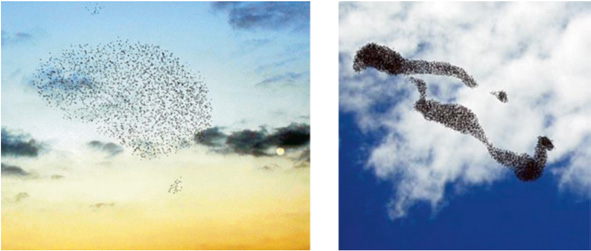
\includegraphics[width = 0.6\linewidth]{Pics/swarm.jpg}
        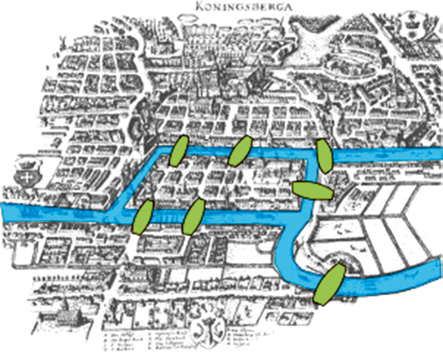
\includegraphics[width = 0.33\linewidth]{Pics/7bridge.jpg}
        \caption{Natural and human complex phenomena. \href{https://link.springer.com/book/10.1007/978-3-319-02024-2}{Source}}
        \label{fig:nathum}
    \end{figure}
\end{frame}